\documentclass{sig-alternate-br}

\begin{document}
\conferenceinfo{13$^{th}$ Twente Student Conference on IT}{June 21$^{st}$, 2010, Enschede, The Netherlands.}
\CopyrightYear{2010} % Allows default copyright year (200X) to be over-ridden - IF NEED BE.

\title{A Multi-Agent System in Haskell}

\numberofauthors{3}
\author{
\alignauthor
Tanja de Jong\\
       \affaddr{University of Twente}\\
       \affaddr{P.O. Box 217, 7500AE Enschede}\\
       \affaddr{The Netherlands}\\
       \email{t.dejong-4@student.utwente.nl}
}

\maketitle
\begin{abstract}
This proposal investigates a multi-agent home automation system in Haskell. As the name implies, a multi-agent system is a system that exists of multiple cooperating agents, that can individually solve problems through reasoning and communicate with each other in order to solve a bigger problem together. A home automation system integrates electrical devices in a house with each other in order to gain a higher quality of living for the residents. Because automation systems consist of multiple appliances and devices that are connected through a network and communicate with each other, a multi-agent system seems a good approach for the implementation of a home automation system. This system will be implemented in the programming language Haskell, which is a functional language. Functional languages are programming languages with a mathematical nature, which relates closely to the logical reasoning that is used by the agents of a multi-agent system.

This research will hopefully result in an answer to the question of how suitable functional languages are for the definition of multi-agent systems.
\end{abstract}

\keywords{Multi-Agent System, Agent, Logic, Reasoning, Functional Language, Haskell, Home Automation System}

\section{Introduction}
\subsection{Multi-Agent System}
A multi-agent system exists of multiple cooperating intelligent agents that can individually solve problems through reasoning and communicate with each other in order to solve a bigger problem together. Multi-agent systems can be used for solving problems that can not -or not as easily- be solved by a single agent or a monolithic system. These types of systems can have several advantages, for example:
\begin{itemize}
\item robustness;
\item scalability;
\item adaptability.
\end{itemize}
Because home automation systems consist of multiple appliances and devices that are connected through a network and communicate with each other, these types of systems are very complex to control in a centralized way \cite{mast}. For this reason, a multi-agent system might be a good approach for defining a home automation system, which is the case that will be used for this research.

\subsection{Haskell}
%WIJZIGINGEN DOORVOEREN
Functional languages are of a mathematical nature, which relates closely to the logical reasoning that is used by the agents of a multi-agent system, and this might have advantages for defining multi-agent systems \cite{dif}. The language of a multi-agent system can be embedded in a functional language and functions for reasoning about the system can be implemented in the same functional language. Therefore, it seems to make sense to define a home automation multi-agent system in such a functional language. Because Haskell is an advanced and widely used functional language, the multi-agent system described in this proposal will be defined in Haskell. 

\subsection{Home Automation}
Home automation is a popular subject nowadays, because of numerous advantages of automation that can add convenience and safety to people's lives. Therefore, a new generation of such systems with even more automation is called for.

Home automation is "a way of integrating technology and services in order to gain a higher quality of living", according to Stichting Smart Homes, Nationaal Kenniscentrum Domotica \& Slim Wonen \cite{ssh}. This is currently a very popular area of research as the number of new home installations are expected to increase enormously, according to Telecom research firm Berg Insight \cite{berginsight} and market research and intelligence firm ABI Research \cite{abi}. Nowadays, home automation systems can range from simple remote controls to complex networks with many different component that can each have their own form of intelligence and automation. The most intelligent systems that are currently in general use need user input through a pc, smart phone or tablet to start their automation processes. Automation results in numerous advantages for people, for example:
\begin{itemize}
\item added convenience/fun/peace of mind: people have to perform less boring tasks themselves
\item timesaving: automation does work that people would have to do otherwise
\item saving money and better for environment: devices can be turned off automatically when nobody's home
\item increased home safety: lights can be turned on automatically when somebody arrives home
\end{itemize}
\subsection{Problem Statement}
Multi-agent systems can be widely used for various applications, among which home automation, and can have many advantages in comparison to single-agent or monolithic systems \cite{cm}.
Because mathematical logic can be used very well for the reasoning and communication that is performed by these multi-agent systems \cite{b:rara} and because functional languages are of a mathematical nature, it seems that a functional language would be a good choice for the definition of a multi-agent system. Proposed here is to investigate how suitable a functional language is for the definition of a multi-agent system, and specifically a home automation system, in Haskell.

\section{Research Questions}
How suitable is Haskell for the definition of a multi-agent system, and in particular for embedding the language of that system in Haskell?
\begin{itemize}
\item How does such a definition in Haskell compare to one or more similar definitions in other programming languages, for certain properties?
\item How well does the mathematical nature of functional languages comply with the logical reasoning of multi-agent systems?
\end{itemize}
It has not yet been decided for which specific properties the suitability of Haskell will be evaluated, that will be done later on during the project. Relevant properties might be the ease of specification, the length of the resulting code, the flexibility and readability of the specification, etcetera.

\section{Background}
\subsection{Multi-agent systems}
Multi-agent systems are systems composed of multiple interacting computing elements, known as {\it agents}. Some of the applications for multi-agent systems are
workflow and business process management,
distributed sensing,
information retrieval and management,
electronic commerce,
human-computer interfaces,
virtual environments,
social simulation, and many more \cite{b:mas}. In such a system, each agent has its own desires and its own set of beliefs about the environment that is gathered using sensors and communication with other agents. The agent will use these beliefs to reason about its desires in order to determine which desires will result in intentions. Through reasoning about these intentions and the gained beliefs, the agent will attempt to achieve its intentions by using actuators and communication with the other agents, as shown in figure \ref{fig:mas}. For this proposal, a multi-agent system consisting of rational agents, that reason according to the Belief-Desire-Intention (BDI) model, is investigated.
\begin{figure}[h]
\centering
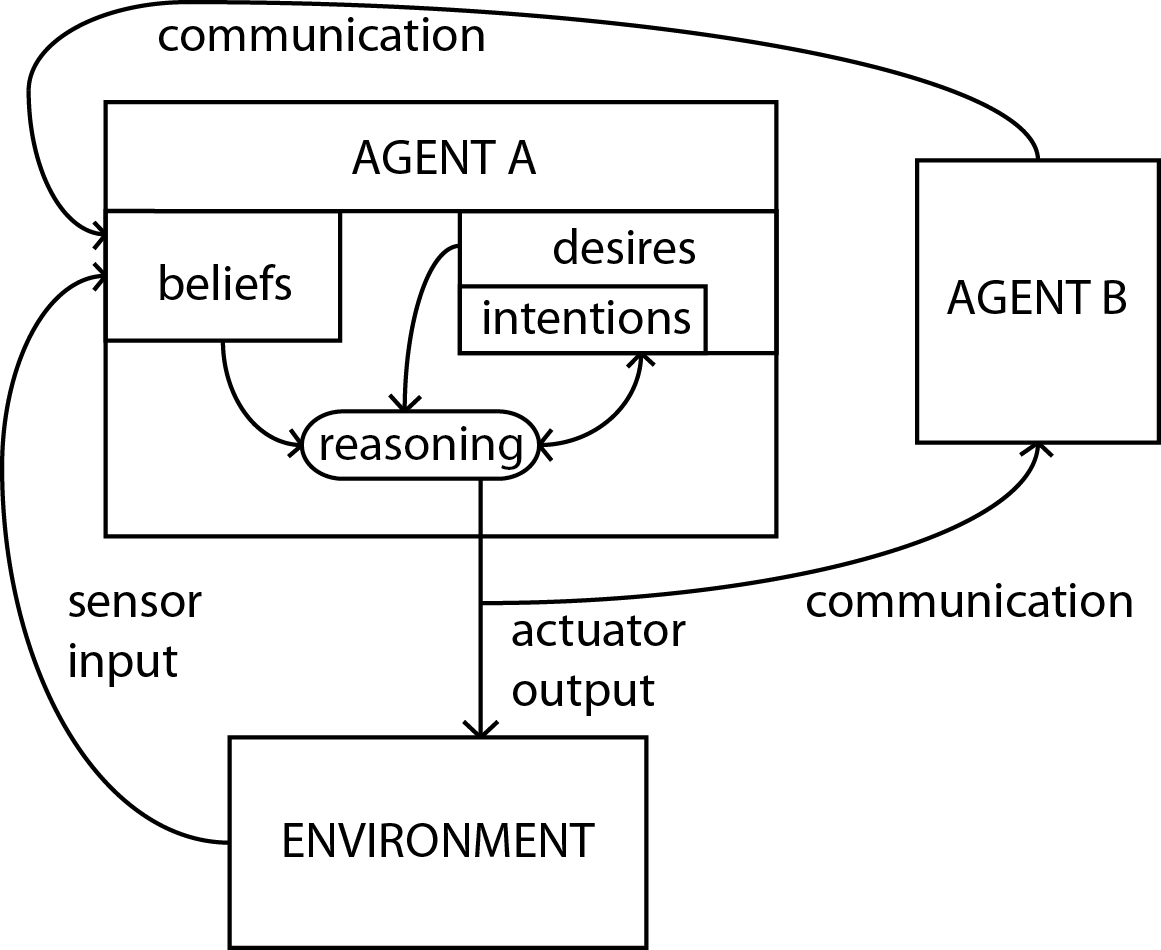
\includegraphics[width=0.45\textwidth]{mas}
\caption{A BDI multi-agent system}
\label{fig:mas}
\end{figure}
\subsubsection{Rational Agents}
According to Wooldridge "an {\it agent} is a computer system that is {\it situated} in some {\it environment}, and that is capable of {\it autonomous} action in this environment in order to meet its design objectives." \cite{b:mas}. Thus, it is an entity that acts upon the environment it inhabits. An agent is said to be rational if it chooses to perform actions that are in its own best interests, given the beliefs it has about the world. Therefore, rational agents are expected to have the following properties, according to Wooldridge and Jennings \cite{b:rara}:
\begin{itemize}
\item autonomy;
\item proactiveness;
\item reactivity; and
\item social ability.
\end{itemize}
\subsubsection{The Belief-Desire-Intention Model}
The Belief-Desire-Intention (BDI) model sees agents' actions as rational in the sense that they are constituted of beliefs, desires, and intentions. The beliefs of an agent correspond to the agent's {\it knowledge} about its environment, but may be incomplete or incorrect. An agents {\it desires} then represent what an agent would want to accomplish and its {\it intentions} represent the desires that it has committed to achieving \cite{b:rara}. This model was originally developed by Michael Bratman \cite{b:ippr}.
\subsubsection{Mathematical logic}
Mathematical logic is a subfield of mathematics that is one of the most important techniques available in computer science and artificial intelligence today. Logic is concerned with the field of reasoning and its correctness and can therefore be used in the engineering of rational agents.  By fixing on a structured, well-defined artificial language it is possible to investigate the question of what can be expressed in a rigorous, mathematical way. This way, any ambiguity can be removed. One of the most desirable features of a software specification language is that it should not dictate how a specification should be satisfied by a definition. A logical specification language has exactly the necessary properties. It does not dictate how a certain agent {\it a} should go about an intention, it is simply expected that {\it a} behaves as a rational agent given such an intention. Therefore, it seems straightforward to define a logical language for the multi-agent system described in this proposal.

\subsection{Functional languages}
Functional languages are of a mathematical nature and have algebraic data types, which result in the possibility for pattern matching. Because of this, agents can reason and communicate using so-called {\it Propositions}, which are statements that can either be true or false. This can be modelled by using algebraic datatypes, which offer the opportunity for pattern matching.
For example, for the home automation system there may be the simplified data type:
-\begin{verbatim}
data Proposition	= PassesBy ComputerAgent HumanAgent
			|  Send Message ComputerAgent ComputerAgent
			|  And Proposition Proposition
			|  Not Proposition
\end{verbatim}
The proposition {\tt PassesBy ComputerAgent HumanAgent} can be used to let another agent know that a certain person, like a resident, has passed by. When another agent receives a message with this particular proposition, it can reason about it and decide if it needs to execute certain actions.

In this scenario, every agent basically consists of a function with its own state that can execute actions and update its state accordingly, whenever a proposition from another agent is received. In the home automation system, these actions may include sending a message to another agent, turning on the radio, etcetera.

By using a functional language for the implementation of a multi-agent system, the language of the multi-agent system can be embedded in Haskell as a datatype and features like pattern matching can be used.

\section{Research Method}
In order to answer the research questions, first of all, research will have to be done to find out whether comparable systems in other languages exist and what the advantages and disadvantages of these languages are. In this case, comparable solutions denote definitions of various multi-agent automation systems that do not necessarily have the exact same functionality as the language that will be defined. After this, it needs to be determined on what properties the systems will be compared and the system can be defined in Haskell. When this is decided, a comparison can be made based on these properties between the system that is defined in Haskell and at least one of the systems that were found in other research. Basically, the research method will consist of these steps:
\begin{itemize}
\item defining a multi-agent home automation system in Haskell as described in this proposal by:
\begin{itemize}
\item implementing an embedded language for the system in Haskell;
\item defining the functions that are used for reasoning within the system in Haskell.
\end{itemize}
\item performing research into existing comparable definitions in other languages;
\item determining on which properties the systems will be compared;

\item compare the newly defined system to the existing systems on the selected properties.
\end{itemize}
\balancecolumns 
\section{Related Work}
There is an extensive amount of research on home automation. However, most of this research does not focus directly on the topic of this proposal.  The degree of automation most common in research needs user input in the form of using a smart phone, computer, or tablet to control the home automation system instead of having the intelligence to automate this. Besides this, there is a lot of focus on energy efficiency, for example by turning of devices when nobody is home \cite{sha}. Although this could of course be accomplished by a higher degree of automation, the focus of the research mentioned in this proposal is on turning on devices when habitants return home, not on turning them off when they leave the house. \cite{mast}

\section{Research Schedule}
\begin{table}[h]
\begin{tabular}{ll}
Date & Description \\ \hline
23-04-2014 & Multi-agent automation system in Haskell defined \\
04-05-2014 & Research on other systems completed \\
11-05-2014 & Properties that will be compared decided \\
25-05-2014 & Comparison of systems completed \\
31-05-2014 & Draft paper finished \\
13-06-2014 & Paper finished \\
\hline\end{tabular}
\end{table}

\bibliographystyle{abbrv}
\bibliography{sigproc}  % sigproc.bib is the name of the Bibliography in this case
% You must have a proper ".bib" file
%  and remember to run:
% latex bibtex latex latex
% to resolve all references
%
% ACM needs 'a single self-contained file'!
%
\vspace{50 mm}
\newpage
\end{document}
